% Options for packages loaded elsewhere
\PassOptionsToPackage{unicode}{hyperref}
\PassOptionsToPackage{hyphens}{url}
\PassOptionsToPackage{dvipsnames,svgnames,x11names}{xcolor}
%
\documentclass[
  letterpaper,
  DIV=11,
  numbers=noendperiod]{scrartcl}

\usepackage{amsmath,amssymb}
\usepackage{iftex}
\ifPDFTeX
  \usepackage[T1]{fontenc}
  \usepackage[utf8]{inputenc}
  \usepackage{textcomp} % provide euro and other symbols
\else % if luatex or xetex
  \usepackage{unicode-math}
  \defaultfontfeatures{Scale=MatchLowercase}
  \defaultfontfeatures[\rmfamily]{Ligatures=TeX,Scale=1}
\fi
\usepackage{lmodern}
\ifPDFTeX\else  
    % xetex/luatex font selection
\fi
% Use upquote if available, for straight quotes in verbatim environments
\IfFileExists{upquote.sty}{\usepackage{upquote}}{}
\IfFileExists{microtype.sty}{% use microtype if available
  \usepackage[]{microtype}
  \UseMicrotypeSet[protrusion]{basicmath} % disable protrusion for tt fonts
}{}
\makeatletter
\@ifundefined{KOMAClassName}{% if non-KOMA class
  \IfFileExists{parskip.sty}{%
    \usepackage{parskip}
  }{% else
    \setlength{\parindent}{0pt}
    \setlength{\parskip}{6pt plus 2pt minus 1pt}}
}{% if KOMA class
  \KOMAoptions{parskip=half}}
\makeatother
\usepackage{xcolor}
\setlength{\emergencystretch}{3em} % prevent overfull lines
\setcounter{secnumdepth}{-\maxdimen} % remove section numbering
% Make \paragraph and \subparagraph free-standing
\ifx\paragraph\undefined\else
  \let\oldparagraph\paragraph
  \renewcommand{\paragraph}[1]{\oldparagraph{#1}\mbox{}}
\fi
\ifx\subparagraph\undefined\else
  \let\oldsubparagraph\subparagraph
  \renewcommand{\subparagraph}[1]{\oldsubparagraph{#1}\mbox{}}
\fi

\usepackage{color}
\usepackage{fancyvrb}
\newcommand{\VerbBar}{|}
\newcommand{\VERB}{\Verb[commandchars=\\\{\}]}
\DefineVerbatimEnvironment{Highlighting}{Verbatim}{commandchars=\\\{\}}
% Add ',fontsize=\small' for more characters per line
\usepackage{framed}
\definecolor{shadecolor}{RGB}{241,243,245}
\newenvironment{Shaded}{\begin{snugshade}}{\end{snugshade}}
\newcommand{\AlertTok}[1]{\textcolor[rgb]{0.68,0.00,0.00}{#1}}
\newcommand{\AnnotationTok}[1]{\textcolor[rgb]{0.37,0.37,0.37}{#1}}
\newcommand{\AttributeTok}[1]{\textcolor[rgb]{0.40,0.45,0.13}{#1}}
\newcommand{\BaseNTok}[1]{\textcolor[rgb]{0.68,0.00,0.00}{#1}}
\newcommand{\BuiltInTok}[1]{\textcolor[rgb]{0.00,0.23,0.31}{#1}}
\newcommand{\CharTok}[1]{\textcolor[rgb]{0.13,0.47,0.30}{#1}}
\newcommand{\CommentTok}[1]{\textcolor[rgb]{0.37,0.37,0.37}{#1}}
\newcommand{\CommentVarTok}[1]{\textcolor[rgb]{0.37,0.37,0.37}{\textit{#1}}}
\newcommand{\ConstantTok}[1]{\textcolor[rgb]{0.56,0.35,0.01}{#1}}
\newcommand{\ControlFlowTok}[1]{\textcolor[rgb]{0.00,0.23,0.31}{#1}}
\newcommand{\DataTypeTok}[1]{\textcolor[rgb]{0.68,0.00,0.00}{#1}}
\newcommand{\DecValTok}[1]{\textcolor[rgb]{0.68,0.00,0.00}{#1}}
\newcommand{\DocumentationTok}[1]{\textcolor[rgb]{0.37,0.37,0.37}{\textit{#1}}}
\newcommand{\ErrorTok}[1]{\textcolor[rgb]{0.68,0.00,0.00}{#1}}
\newcommand{\ExtensionTok}[1]{\textcolor[rgb]{0.00,0.23,0.31}{#1}}
\newcommand{\FloatTok}[1]{\textcolor[rgb]{0.68,0.00,0.00}{#1}}
\newcommand{\FunctionTok}[1]{\textcolor[rgb]{0.28,0.35,0.67}{#1}}
\newcommand{\ImportTok}[1]{\textcolor[rgb]{0.00,0.46,0.62}{#1}}
\newcommand{\InformationTok}[1]{\textcolor[rgb]{0.37,0.37,0.37}{#1}}
\newcommand{\KeywordTok}[1]{\textcolor[rgb]{0.00,0.23,0.31}{#1}}
\newcommand{\NormalTok}[1]{\textcolor[rgb]{0.00,0.23,0.31}{#1}}
\newcommand{\OperatorTok}[1]{\textcolor[rgb]{0.37,0.37,0.37}{#1}}
\newcommand{\OtherTok}[1]{\textcolor[rgb]{0.00,0.23,0.31}{#1}}
\newcommand{\PreprocessorTok}[1]{\textcolor[rgb]{0.68,0.00,0.00}{#1}}
\newcommand{\RegionMarkerTok}[1]{\textcolor[rgb]{0.00,0.23,0.31}{#1}}
\newcommand{\SpecialCharTok}[1]{\textcolor[rgb]{0.37,0.37,0.37}{#1}}
\newcommand{\SpecialStringTok}[1]{\textcolor[rgb]{0.13,0.47,0.30}{#1}}
\newcommand{\StringTok}[1]{\textcolor[rgb]{0.13,0.47,0.30}{#1}}
\newcommand{\VariableTok}[1]{\textcolor[rgb]{0.07,0.07,0.07}{#1}}
\newcommand{\VerbatimStringTok}[1]{\textcolor[rgb]{0.13,0.47,0.30}{#1}}
\newcommand{\WarningTok}[1]{\textcolor[rgb]{0.37,0.37,0.37}{\textit{#1}}}

\providecommand{\tightlist}{%
  \setlength{\itemsep}{0pt}\setlength{\parskip}{0pt}}\usepackage{longtable,booktabs,array}
\usepackage{calc} % for calculating minipage widths
% Correct order of tables after \paragraph or \subparagraph
\usepackage{etoolbox}
\makeatletter
\patchcmd\longtable{\par}{\if@noskipsec\mbox{}\fi\par}{}{}
\makeatother
% Allow footnotes in longtable head/foot
\IfFileExists{footnotehyper.sty}{\usepackage{footnotehyper}}{\usepackage{footnote}}
\makesavenoteenv{longtable}
\usepackage{graphicx}
\makeatletter
\def\maxwidth{\ifdim\Gin@nat@width>\linewidth\linewidth\else\Gin@nat@width\fi}
\def\maxheight{\ifdim\Gin@nat@height>\textheight\textheight\else\Gin@nat@height\fi}
\makeatother
% Scale images if necessary, so that they will not overflow the page
% margins by default, and it is still possible to overwrite the defaults
% using explicit options in \includegraphics[width, height, ...]{}
\setkeys{Gin}{width=\maxwidth,height=\maxheight,keepaspectratio}
% Set default figure placement to htbp
\makeatletter
\def\fps@figure{htbp}
\makeatother

\KOMAoption{captions}{tableheading}
\makeatletter
\makeatother
\makeatletter
\makeatother
\makeatletter
\@ifpackageloaded{caption}{}{\usepackage{caption}}
\AtBeginDocument{%
\ifdefined\contentsname
  \renewcommand*\contentsname{Table of contents}
\else
  \newcommand\contentsname{Table of contents}
\fi
\ifdefined\listfigurename
  \renewcommand*\listfigurename{List of Figures}
\else
  \newcommand\listfigurename{List of Figures}
\fi
\ifdefined\listtablename
  \renewcommand*\listtablename{List of Tables}
\else
  \newcommand\listtablename{List of Tables}
\fi
\ifdefined\figurename
  \renewcommand*\figurename{Figure}
\else
  \newcommand\figurename{Figure}
\fi
\ifdefined\tablename
  \renewcommand*\tablename{Table}
\else
  \newcommand\tablename{Table}
\fi
}
\@ifpackageloaded{float}{}{\usepackage{float}}
\floatstyle{ruled}
\@ifundefined{c@chapter}{\newfloat{codelisting}{h}{lop}}{\newfloat{codelisting}{h}{lop}[chapter]}
\floatname{codelisting}{Listing}
\newcommand*\listoflistings{\listof{codelisting}{List of Listings}}
\makeatother
\makeatletter
\@ifpackageloaded{caption}{}{\usepackage{caption}}
\@ifpackageloaded{subcaption}{}{\usepackage{subcaption}}
\makeatother
\makeatletter
\@ifpackageloaded{tcolorbox}{}{\usepackage[skins,breakable]{tcolorbox}}
\makeatother
\makeatletter
\@ifundefined{shadecolor}{\definecolor{shadecolor}{rgb}{.97, .97, .97}}
\makeatother
\makeatletter
\makeatother
\makeatletter
\makeatother
\ifLuaTeX
  \usepackage{selnolig}  % disable illegal ligatures
\fi
\IfFileExists{bookmark.sty}{\usepackage{bookmark}}{\usepackage{hyperref}}
\IfFileExists{xurl.sty}{\usepackage{xurl}}{} % add URL line breaks if available
\urlstyle{same} % disable monospaced font for URLs
\hypersetup{
  pdftitle={FYS-STK Exercises week 35},
  colorlinks=true,
  linkcolor={blue},
  filecolor={Maroon},
  citecolor={Blue},
  urlcolor={Blue},
  pdfcreator={LaTeX via pandoc}}

\title{FYS-STK Exercises week 35}
\author{}
\date{}

\begin{document}
\maketitle
\ifdefined\Shaded\renewenvironment{Shaded}{\begin{tcolorbox}[sharp corners, boxrule=0pt, interior hidden, enhanced, borderline west={3pt}{0pt}{shadecolor}, breakable, frame hidden]}{\end{tcolorbox}}\fi

\begin{Shaded}
\begin{Highlighting}[]
\ImportTok{import}\NormalTok{ numpy }\ImportTok{as}\NormalTok{ np}
\ImportTok{import}\NormalTok{ matplotlib.pyplot }\ImportTok{as}\NormalTok{ plt}
\end{Highlighting}
\end{Shaded}

\hypertarget{exercise-2}{%
\subsection{Exercise 2}\label{exercise-2}}

First we create our random x, and a dependent y with noise drawn from a
normal distribution with standard deviation 0.1 (code modified from the
exercise text).

\begin{Shaded}
\begin{Highlighting}[]
\NormalTok{np.random.seed(}\DecValTok{10}\NormalTok{)}
\NormalTok{x }\OperatorTok{=}\NormalTok{ np.random.rand(}\DecValTok{100}\NormalTok{,}\DecValTok{1}\NormalTok{)}
\NormalTok{noise }\OperatorTok{=} \FloatTok{0.1} \OperatorTok{*}\NormalTok{ np.random.randn(}\DecValTok{100}\NormalTok{,}\DecValTok{1}\NormalTok{)}
\NormalTok{y }\OperatorTok{=} \FloatTok{2.0}\OperatorTok{+}\DecValTok{5}\OperatorTok{*}\NormalTok{x}\OperatorTok{*}\NormalTok{x }\OperatorTok{+}\NormalTok{ noise}
\end{Highlighting}
\end{Shaded}

Then we create our design matrix, with intercept, and x up to the second
power.

\begin{Shaded}
\begin{Highlighting}[]
\NormalTok{X }\OperatorTok{=}\NormalTok{ np.zeros((}\DecValTok{100}\NormalTok{,}\DecValTok{3}\NormalTok{))}
\NormalTok{X[:,}\DecValTok{0}\NormalTok{] }\OperatorTok{=} \DecValTok{1}
\NormalTok{X[:,}\DecValTok{1}\NormalTok{] }\OperatorTok{=}\NormalTok{ x.T}
\NormalTok{X[:,}\DecValTok{2}\NormalTok{] }\OperatorTok{=}\NormalTok{ (x}\OperatorTok{**}\DecValTok{2}\NormalTok{).T}
\end{Highlighting}
\end{Shaded}

Then we optimize the cost function, here mean squared error (MSE), to
get our betas with the analytical expression

\[
\boldsymbol{\beta} =\left(\boldsymbol{X}^T\boldsymbol{X}\right)^{-1}\boldsymbol{X}^T\boldsymbol{y}.
\]

\begin{Shaded}
\begin{Highlighting}[]
\CommentTok{\# optimize MSE}
\NormalTok{xtx\_inv }\OperatorTok{=}\NormalTok{ np.linalg.inv(X.T.dot(X))}

\NormalTok{Best }\OperatorTok{=}\NormalTok{ xtx\_inv.dot(X.T).dot(y)}
\BuiltInTok{print}\NormalTok{(}\SpecialStringTok{f"Beta vector: }\SpecialCharTok{\{}\NormalTok{Best}\SpecialCharTok{.}\NormalTok{T}\SpecialCharTok{\}}\SpecialStringTok{"}\NormalTok{)}
\end{Highlighting}
\end{Shaded}

\begin{verbatim}
Beta vector: [[2.0146372  0.02474757 4.93762474]]
\end{verbatim}

We then get our predicted \(\boldsymbol{\widetilde{y}}\) using

\[
\boldsymbol{\tilde{y}}= \boldsymbol{X}\boldsymbol{\beta},
\]

\begin{Shaded}
\begin{Highlighting}[]
\NormalTok{ytilde }\OperatorTok{=}\NormalTok{ X.dot(Best)}
\end{Highlighting}
\end{Shaded}

and calculate MSE

\[
MSE(\boldsymbol{y},\boldsymbol{\tilde{y}}) = \frac{1}{n}
\sum_{i=0}^{n-1}(y_i-\tilde{y}_i)^2.
\]

\begin{Shaded}
\begin{Highlighting}[]
\NormalTok{MSE }\OperatorTok{=} \BuiltInTok{sum}\NormalTok{((y }\OperatorTok{{-}}\NormalTok{ ytilde)}\OperatorTok{**}\DecValTok{2}\NormalTok{) }\OperatorTok{/} \BuiltInTok{len}\NormalTok{(y)}
\BuiltInTok{print}\NormalTok{(}\SpecialStringTok{f"MSE: }\SpecialCharTok{\{}\BuiltInTok{round}\NormalTok{(MSE.item(), }\DecValTok{5}\NormalTok{)}\SpecialCharTok{\}}\SpecialStringTok{"}\NormalTok{)}
\end{Highlighting}
\end{Shaded}

\begin{verbatim}
MSE: 0.00971
\end{verbatim}

The MSE is 0.00971, which is very close to the value 0.1 that we used
for our simulation.

Finally, we plot the data and regression

\begin{Shaded}
\begin{Highlighting}[]
\NormalTok{sorted\_index }\OperatorTok{=}\NormalTok{ np.argsort(x, axis}\OperatorTok{=}\VariableTok{None}\NormalTok{)}
\CommentTok{\#print(sorted\_index)}
\NormalTok{xsort }\OperatorTok{=}\NormalTok{ x[sorted\_index]}
\NormalTok{ysort }\OperatorTok{=}\NormalTok{ y[sorted\_index]}
\NormalTok{ytsort }\OperatorTok{=}\NormalTok{ ytilde[sorted\_index]}

\NormalTok{plt.plot(xsort, ysort, }\StringTok{"."}\NormalTok{)}
\NormalTok{plt.plot(xsort, ytsort, }\StringTok{"{-}"}\NormalTok{, label }\OperatorTok{=} \StringTok{"Line of best fit"}\NormalTok{)}
\NormalTok{plt.xlabel(}\StringTok{"x"}\NormalTok{)}
\NormalTok{plt.ylabel(}\StringTok{"y"}\NormalTok{)}
\NormalTok{plt.legend()}
\NormalTok{plt.show()}
\end{Highlighting}
\end{Shaded}

\begin{figure}[H]

{\centering 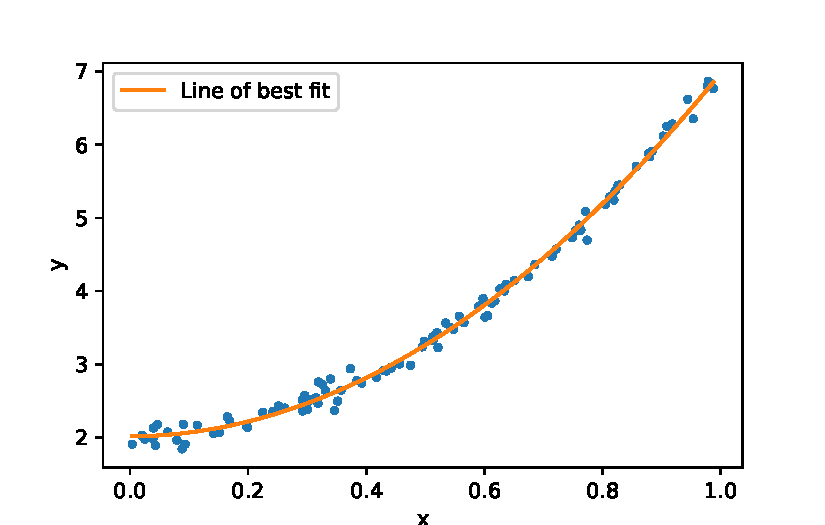
\includegraphics{w35-exercises_files/figure-pdf/unnamed-chunk-7-1.pdf}

}

\caption{Linear regression for a model fit with polynomials up to the
second degree.}

\end{figure}

\hypertarget{exercise-3}{%
\subsection{Exercise 3}\label{exercise-3}}

\hypertarget{a}{%
\subsubsection{a)}\label{a}}

For this exercise we also import \texttt{train\_test\_split} from
\texttt{sklearn}.

\begin{Shaded}
\begin{Highlighting}[]
\ImportTok{from}\NormalTok{ sklearn.model\_selection }\ImportTok{import}\NormalTok{ train\_test\_split}
\end{Highlighting}
\end{Shaded}

Create data (code from the exercise text)

\begin{Shaded}
\begin{Highlighting}[]
\NormalTok{np.random.seed()}
\NormalTok{n }\OperatorTok{=} \DecValTok{100}
\CommentTok{\# Make data set.}
\NormalTok{x }\OperatorTok{=}\NormalTok{ np.linspace(}\OperatorTok{{-}}\DecValTok{3}\NormalTok{, }\DecValTok{3}\NormalTok{, n).reshape(}\OperatorTok{{-}}\DecValTok{1}\NormalTok{, }\DecValTok{1}\NormalTok{)}
\NormalTok{y }\OperatorTok{=}\NormalTok{ np.exp(}\OperatorTok{{-}}\NormalTok{x}\OperatorTok{**}\DecValTok{2}\NormalTok{) }\OperatorTok{+} \FloatTok{1.5} \OperatorTok{*}\NormalTok{ np.exp(}\OperatorTok{{-}}\NormalTok{(x}\OperatorTok{{-}}\DecValTok{2}\NormalTok{)}\OperatorTok{**}\DecValTok{2}\NormalTok{)}\OperatorTok{+}\NormalTok{ np.random.normal(}\DecValTok{0}\NormalTok{, }\FloatTok{0.1}\NormalTok{, x.shape)}
\end{Highlighting}
\end{Shaded}

Create a function to make a design matrix with an nth order polynomial

\begin{Shaded}
\begin{Highlighting}[]
\KeywordTok{def}\NormalTok{ design\_poly\_n(x, n):}
\NormalTok{    X }\OperatorTok{=}\NormalTok{ np.zeros((}\BuiltInTok{len}\NormalTok{(x), n))}
\NormalTok{    X[:,}\DecValTok{0}\NormalTok{] }\OperatorTok{=} \DecValTok{1}
    \ControlFlowTok{for}\NormalTok{ i }\KeywordTok{in} \BuiltInTok{range}\NormalTok{(}\DecValTok{1}\NormalTok{, n):}
\NormalTok{        X[:,i] }\OperatorTok{=}\NormalTok{ (x}\OperatorTok{**}\NormalTok{i).T}

    \ControlFlowTok{return}\NormalTok{ X}
\end{Highlighting}
\end{Shaded}

Then create design matrix up to a 5th order polynomial, and split in
training and test data

\begin{Shaded}
\begin{Highlighting}[]
\NormalTok{X }\OperatorTok{=}\NormalTok{ design\_poly\_n(x, }\DecValTok{5}\NormalTok{)}
\NormalTok{X\_train, X\_test, y\_train, y\_test }\OperatorTok{=}\NormalTok{ train\_test\_split(X, y, test\_size}\OperatorTok{=}\FloatTok{0.2}\NormalTok{)}
\end{Highlighting}
\end{Shaded}

\hypertarget{b}{%
\subsection{b)}\label{b}}

Calculate optimal beta and MSE

\begin{Shaded}
\begin{Highlighting}[]
\NormalTok{xtx\_inv }\OperatorTok{=}\NormalTok{ np.linalg.inv(X\_train.T.dot(X\_train))}
\NormalTok{Best }\OperatorTok{=}\NormalTok{ xtx\_inv.dot(X\_train.T).dot(y\_train)}
\BuiltInTok{print}\NormalTok{(}\StringTok{"Beta:"}\NormalTok{, Best.T)}
\end{Highlighting}
\end{Shaded}

\begin{verbatim}
Beta: [[ 0.8626045   0.44595956 -0.01713606 -0.03636564 -0.00540025]]
\end{verbatim}

\begin{Shaded}
\begin{Highlighting}[]
\NormalTok{ytilde\_train }\OperatorTok{=}\NormalTok{ X\_train.dot(Best)}
\NormalTok{MSE }\OperatorTok{=} \BuiltInTok{sum}\NormalTok{((y\_train }\OperatorTok{{-}}\NormalTok{ ytilde\_train)}\OperatorTok{**}\DecValTok{2}\NormalTok{) }\OperatorTok{/} \BuiltInTok{len}\NormalTok{(y\_train)}
\BuiltInTok{print}\NormalTok{(}\StringTok{"MSE"}\NormalTok{, MSE)}
\end{Highlighting}
\end{Shaded}

\begin{verbatim}
MSE [0.02859804]
\end{verbatim}

Compare to MSE when applying betas from training data to test data

\begin{Shaded}
\begin{Highlighting}[]
\NormalTok{ytilde\_test }\OperatorTok{=}\NormalTok{ X\_test.dot(Best)}
\NormalTok{MSE }\OperatorTok{=} \BuiltInTok{sum}\NormalTok{((y\_test }\OperatorTok{{-}}\NormalTok{ ytilde\_test)}\OperatorTok{**}\DecValTok{2}\NormalTok{) }\OperatorTok{/} \BuiltInTok{len}\NormalTok{(y\_test)}
\BuiltInTok{print}\NormalTok{(}\StringTok{"MSE"}\NormalTok{, MSE)}
\end{Highlighting}
\end{Shaded}

\begin{verbatim}
MSE [0.02913716]
\end{verbatim}

MSE is a bit higher for the test data.

\hypertarget{c}{%
\subsubsection{c)}\label{c}}

\begin{Shaded}
\begin{Highlighting}[]
\NormalTok{np.random.seed(}\DecValTok{3489}\NormalTok{)}
\NormalTok{n }\OperatorTok{=} \DecValTok{100}
\CommentTok{\# Make data set.}
\NormalTok{x }\OperatorTok{=}\NormalTok{ np.linspace(}\OperatorTok{{-}}\DecValTok{3}\NormalTok{, }\DecValTok{3}\NormalTok{, n).reshape(}\OperatorTok{{-}}\DecValTok{1}\NormalTok{, }\DecValTok{1}\NormalTok{)}
\NormalTok{y }\OperatorTok{=}\NormalTok{ np.exp(}\OperatorTok{{-}}\NormalTok{x}\OperatorTok{**}\DecValTok{2}\NormalTok{) }\OperatorTok{+} \FloatTok{1.5} \OperatorTok{*}\NormalTok{ np.exp(}\OperatorTok{{-}}\NormalTok{(x}\OperatorTok{{-}}\DecValTok{2}\NormalTok{)}\OperatorTok{**}\DecValTok{2}\NormalTok{)}\OperatorTok{+}\NormalTok{ np.random.normal(}\DecValTok{0}\NormalTok{, }\FloatTok{0.1}\NormalTok{, x.shape)}

\NormalTok{maxpoly }\OperatorTok{=} \DecValTok{15}
\NormalTok{poly }\OperatorTok{=}\NormalTok{ np.arange(maxpoly) }\OperatorTok{+} \DecValTok{1}
\NormalTok{MSE\_train\_out }\OperatorTok{=}\NormalTok{ np.zeros(maxpoly)}
\NormalTok{MSE\_test\_out }\OperatorTok{=}\NormalTok{ np.zeros(maxpoly)}

\ControlFlowTok{for}\NormalTok{ i }\KeywordTok{in}\NormalTok{ poly:}
\NormalTok{    X }\OperatorTok{=}\NormalTok{ design\_poly\_n(x, i)}
\NormalTok{    X\_train, X\_test, y\_train, y\_test }\OperatorTok{=}\NormalTok{ train\_test\_split(X, y, test\_size}\OperatorTok{=}\FloatTok{0.2}\NormalTok{)}
\NormalTok{    xtx\_inv }\OperatorTok{=}\NormalTok{ np.linalg.inv(X\_train.T.dot(X\_train))}
\NormalTok{    Best }\OperatorTok{=}\NormalTok{ xtx\_inv.dot(X\_train.T).dot(y\_train)}
    
\NormalTok{    ytilde\_train }\OperatorTok{=}\NormalTok{ X\_train.dot(Best)}
\NormalTok{    MSE\_train\_out[i}\OperatorTok{{-}}\DecValTok{1}\NormalTok{] }\OperatorTok{=} \BuiltInTok{sum}\NormalTok{((y\_train }\OperatorTok{{-}}\NormalTok{ ytilde\_train)}\OperatorTok{**}\DecValTok{2}\NormalTok{) }\OperatorTok{/} \BuiltInTok{len}\NormalTok{(y\_train)}
    
\NormalTok{    ytilde\_test }\OperatorTok{=}\NormalTok{ X\_test.dot(Best)}
\NormalTok{    MSE\_test\_out[i}\OperatorTok{{-}}\DecValTok{1}\NormalTok{] }\OperatorTok{=} \BuiltInTok{sum}\NormalTok{((y\_test }\OperatorTok{{-}}\NormalTok{ ytilde\_test)}\OperatorTok{**}\DecValTok{2}\NormalTok{) }\OperatorTok{/} \BuiltInTok{len}\NormalTok{(y\_test)}
\end{Highlighting}
\end{Shaded}

Then plot the MSEs to compare test and train set. Passing on to R for
plotting.

\begin{Shaded}
\begin{Highlighting}[]
\CommentTok{\# R code}
\CommentTok{\# passing onto R for plotting }
\FunctionTok{library}\NormalTok{(reticulate)}
\FunctionTok{library}\NormalTok{(tidyverse)}

\NormalTok{polydeg }\OtherTok{\textless{}{-}}\NormalTok{ py}\SpecialCharTok{$}\NormalTok{poly}
\NormalTok{MSEtest }\OtherTok{\textless{}{-}}\NormalTok{ py}\SpecialCharTok{$}\NormalTok{MSE\_test\_out}
\NormalTok{MSEtrain }\OtherTok{\textless{}{-}}\NormalTok{ py}\SpecialCharTok{$}\NormalTok{MSE\_train\_out}

\NormalTok{df }\OtherTok{\textless{}{-}} \FunctionTok{data.frame}\NormalTok{(}
    \AttributeTok{poly =}\NormalTok{ polydeg,}
    \AttributeTok{test =}\NormalTok{ MSEtest,}
    \AttributeTok{train =}\NormalTok{ MSEtrain}
\NormalTok{) }\SpecialCharTok{\%\textgreater{}\%}
    \FunctionTok{pivot\_longer}\NormalTok{(}\FunctionTok{c}\NormalTok{(test,train), }\AttributeTok{names\_to =} \StringTok{"data\_type"}\NormalTok{, }\AttributeTok{values\_to =} \StringTok{"MSE"}\NormalTok{)}

\FunctionTok{ggplot}\NormalTok{(df, }\FunctionTok{aes}\NormalTok{(poly, MSE, }\AttributeTok{col =}\NormalTok{ data\_type)) }\SpecialCharTok{+}
    \FunctionTok{geom\_line}\NormalTok{() }\SpecialCharTok{+}
    \FunctionTok{theme\_bw}\NormalTok{() }\SpecialCharTok{+}
    \FunctionTok{labs}\NormalTok{(}
        \AttributeTok{x =} \StringTok{"Polynomial degree"}\NormalTok{,}
        \AttributeTok{color =} \StringTok{"Data type"}
\NormalTok{    )}
\end{Highlighting}
\end{Shaded}

\begin{figure}[H]

{\centering 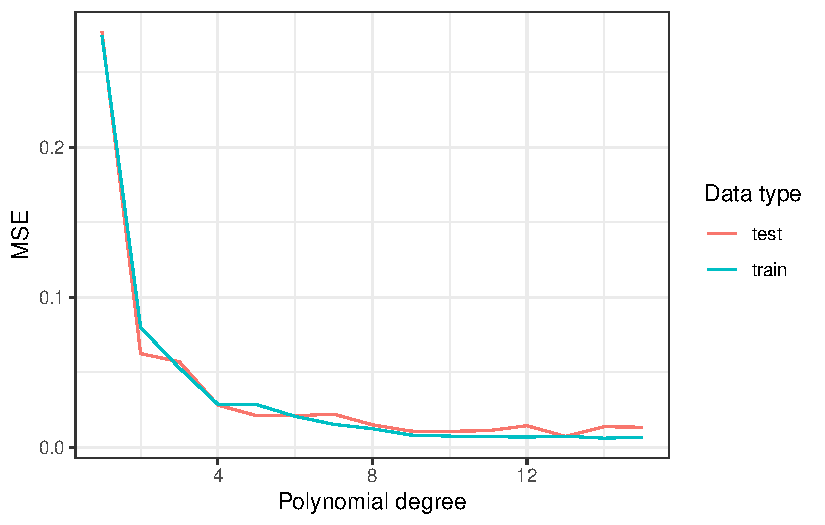
\includegraphics{w35-exercises_files/figure-pdf/unnamed-chunk-15-3.pdf}

}

\caption{MSE as function of highest polynomial degree included in the
model for training (80\%) and test (20\%) data. n = 100}

\end{figure}

For 15 degree polynomials the the test and training are still pretty
similar. MSE for the training data is decreasing for each polynomial
degree, while for the test data it fluctuates a bit more, the minimum
seemingly at 13 degrees.

Try a higher-degree polynomial

\begin{Shaded}
\begin{Highlighting}[]

\NormalTok{np.random.seed(}\DecValTok{3489}\NormalTok{)}
\NormalTok{n }\OperatorTok{=} \DecValTok{100}
\CommentTok{\# Make data set.}
\NormalTok{x }\OperatorTok{=}\NormalTok{ np.linspace(}\OperatorTok{{-}}\DecValTok{3}\NormalTok{, }\DecValTok{3}\NormalTok{, n).reshape(}\OperatorTok{{-}}\DecValTok{1}\NormalTok{, }\DecValTok{1}\NormalTok{)}
\NormalTok{y }\OperatorTok{=}\NormalTok{ np.exp(}\OperatorTok{{-}}\NormalTok{x}\OperatorTok{**}\DecValTok{2}\NormalTok{) }\OperatorTok{+} \FloatTok{1.5} \OperatorTok{*}\NormalTok{ np.exp(}\OperatorTok{{-}}\NormalTok{(x}\OperatorTok{{-}}\DecValTok{2}\NormalTok{)}\OperatorTok{**}\DecValTok{2}\NormalTok{)}\OperatorTok{+}\NormalTok{ np.random.normal(}\DecValTok{0}\NormalTok{, }\FloatTok{0.1}\NormalTok{, x.shape)}

\NormalTok{maxpoly }\OperatorTok{=} \DecValTok{20}
\NormalTok{poly }\OperatorTok{=}\NormalTok{ np.arange(maxpoly) }\OperatorTok{+} \DecValTok{1}
\NormalTok{MSE\_train\_out }\OperatorTok{=}\NormalTok{ np.zeros(maxpoly)}
\NormalTok{MSE\_test\_out }\OperatorTok{=}\NormalTok{ np.zeros(maxpoly)}

\ControlFlowTok{for}\NormalTok{ i }\KeywordTok{in}\NormalTok{ poly:}
\NormalTok{    X }\OperatorTok{=}\NormalTok{ design\_poly\_n(x, i)}
\NormalTok{    X\_train, X\_test, y\_train, y\_test }\OperatorTok{=}\NormalTok{ train\_test\_split(X, y, test\_size}\OperatorTok{=}\FloatTok{0.2}\NormalTok{)}
\NormalTok{    xtx\_inv }\OperatorTok{=}\NormalTok{ np.linalg.inv(X\_train.T.dot(X\_train))}
\NormalTok{    Best }\OperatorTok{=}\NormalTok{ xtx\_inv.dot(X\_train.T).dot(y\_train)}
    
\NormalTok{    ytilde\_train }\OperatorTok{=}\NormalTok{ X\_train.dot(Best)}
\NormalTok{    MSE\_train\_out[i}\OperatorTok{{-}}\DecValTok{1}\NormalTok{] }\OperatorTok{=} \BuiltInTok{sum}\NormalTok{((y\_train }\OperatorTok{{-}}\NormalTok{ ytilde\_train)}\OperatorTok{**}\DecValTok{2}\NormalTok{) }\OperatorTok{/} \BuiltInTok{len}\NormalTok{(y\_train)}
    
\NormalTok{    ytilde\_test }\OperatorTok{=}\NormalTok{ X\_test.dot(Best)}
\NormalTok{    MSE\_test\_out[i}\OperatorTok{{-}}\DecValTok{1}\NormalTok{] }\OperatorTok{=} \BuiltInTok{sum}\NormalTok{((y\_test }\OperatorTok{{-}}\NormalTok{ ytilde\_test)}\OperatorTok{**}\DecValTok{2}\NormalTok{) }\OperatorTok{/} \BuiltInTok{len}\NormalTok{(y\_test)}
\end{Highlighting}
\end{Shaded}

\begin{Shaded}
\begin{Highlighting}[]
\CommentTok{\# R code}
\CommentTok{\# passing onto R for plotting }

\NormalTok{polydeg }\OtherTok{\textless{}{-}}\NormalTok{ py}\SpecialCharTok{$}\NormalTok{poly}
\NormalTok{MSEtest }\OtherTok{\textless{}{-}}\NormalTok{ py}\SpecialCharTok{$}\NormalTok{MSE\_test\_out}
\NormalTok{MSEtrain }\OtherTok{\textless{}{-}}\NormalTok{ py}\SpecialCharTok{$}\NormalTok{MSE\_train\_out}

\NormalTok{df }\OtherTok{\textless{}{-}} \FunctionTok{data.frame}\NormalTok{(}
    \AttributeTok{poly =}\NormalTok{ polydeg,}
    \AttributeTok{test =}\NormalTok{ MSEtest,}
    \AttributeTok{train =}\NormalTok{ MSEtrain}
\NormalTok{) }\SpecialCharTok{\%\textgreater{}\%}
    \FunctionTok{pivot\_longer}\NormalTok{(}\FunctionTok{c}\NormalTok{(test,train), }\AttributeTok{names\_to =} \StringTok{"data\_type"}\NormalTok{, }\AttributeTok{values\_to =} \StringTok{"MSE"}\NormalTok{)}

\FunctionTok{ggplot}\NormalTok{(df, }\FunctionTok{aes}\NormalTok{(poly, MSE, }\AttributeTok{col =}\NormalTok{ data\_type)) }\SpecialCharTok{+}
    \FunctionTok{geom\_line}\NormalTok{() }\SpecialCharTok{+}
    \FunctionTok{theme\_bw}\NormalTok{() }\SpecialCharTok{+}
    \FunctionTok{labs}\NormalTok{(}
        \AttributeTok{x =} \StringTok{"Polynomial degree"}\NormalTok{,}
        \AttributeTok{color =} \StringTok{"Data type"}
\NormalTok{    )}
\end{Highlighting}
\end{Shaded}

\begin{figure}[H]

{\centering 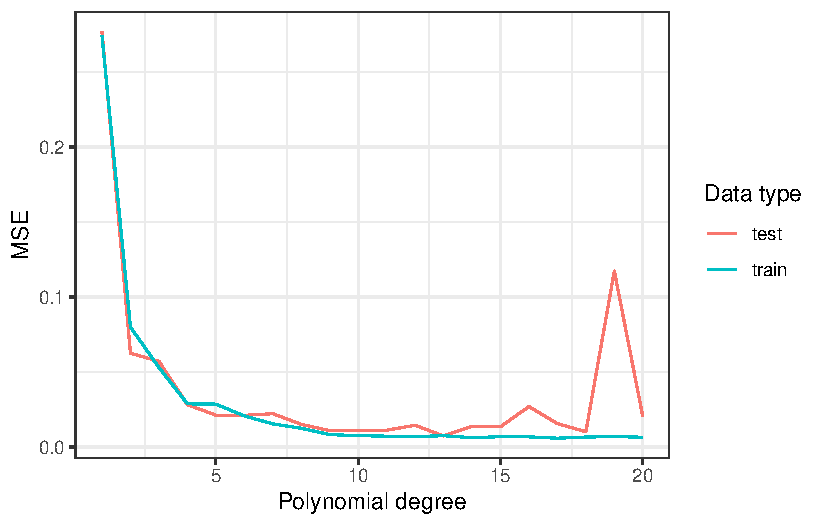
\includegraphics{w35-exercises_files/figure-pdf/unnamed-chunk-17-1.pdf}

}

\caption{MSE as function of highest polynomial degree included in the
model for training (80\%) and test (20\%) data. Same data as the
previous figure, but for a higher polynomial degree. n = 100}

\end{figure}

The MSE starts to really deviate when polynomial degree goes above
around 15. The best trade-off to avoid overfitting is probably around
10-15 degrees.



\end{document}
